\documentclass{standalone}
\usepackage{tikz}
\usetikzlibrary{arrows.meta}
\begin{document}

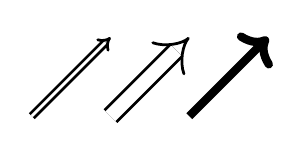
\begin{tikzpicture}  
  \draw[-Implies,line width=1pt,double distance=1pt] (0,0) -- (1,1);
  \draw[-Implies,line width=1pt,double distance=5pt] (1,0) -- (2,1);
  \draw[->,line width=3pt] (2,0) -- (3,1);
\end{tikzpicture}


\begin{tikzpicture}
  [ my double arrow/.style={double distance=2.5mm,
    -{Latex[length=12mm,open]}, line width=1mm,green,
    postaction={draw,double distance=.5mm,line width=1mm, white,-,
      shorten >=10mm}}, ]

  \draw[my double arrow] (0,1) to (4,1);

  \draw[my double arrow, red] (0,0) to (4,0);

\end{tikzpicture}

\end{document}

%%% Local Variables:
%%% mode: latex
%%% TeX-master: t
%%% End:
